\section{Introduction}

% Start with a little story
\begin{center}
  \fbox{
    \parbox{0.85\linewidth}{
    \noindent
    \emph{``What did you see in this image?''\\
      ``Panda, Tiger, Elephant, Lions.''\\
      ``Have you seen the Gorilla?''\\
      ``Oh! I even didn't notice there is a Gorilla !''}
    }
  }
\end{center}

\setlength{\tabcolsep}{2pt}
\begin{figure}[htb]
\begin{center}
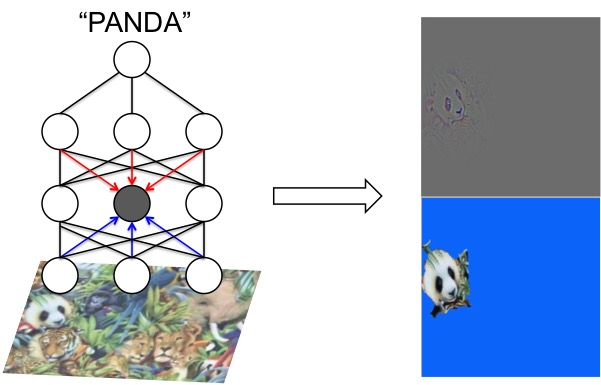
\includegraphics[width=0.9\columnwidth]{figs/splash0/splash}
\caption{Feedback Convolutional Net model for capturing visual attention by inferring the status of hidden neuron activations. It is designed to utilize both bottom-up image inputs and top-down semantic labels to infer the hidden neuron activations. Salient areas captured by feedback often correspond to related ``target'' objects, even in images with cluttered background and multiple objects.}
\label{fig:splash0}
\end{center}
\end{figure}

Visual attention typically is dominated by \emph{``goals''} from our mind easily in a top-down manner, especially in the case of object detection. Cognitive science explains this in the ``Biased Competition Theory''~\cite{beck2009top,desimone1998visual,desimone1995neural}, that human visual cortex is enhanced by top-down stimuli and non-relevant neurons will be suppressed in feedback loops when searching for objects. By ``\emph{looking and thinking twice}'', both human recognition and detection performances increase significantly, especially in images with cluttered background~\cite{Cichy2014Resolving}. This leads to the selectivity in neuron activations~\cite{Kruger2013Deep}, which reduces the chance of recognition being interfered with either noises or distractive patterns.

Inspired by above evidences, we present a novel \emph{Feedback Convolutional Neural Network} architecture in this paper. It achieves this selectivity by jointly reasoning outputs of class nodes and activations of hidden layer neurons during the feedback loop. As shown in Figure~\ref{fig:splash0}, during the feedforward stage, the proposed networks perform inference from input images in a bottom-up manner as traditional Convolutional Networks; while in feedback loops, it sets up high-level semantic labels, (\emph{e.g.}, outputs of class nodes) as the ``goal'' in visual search to infer the activation status of hidden layer neurons. We show that the network is powerful enough to apply for class model visualization~\cite{simonyan2013deep, zeiler2014visualizing}, object localization~\cite{simonyan2013deep} and image classification~\cite{Krizhevsky2012ImageNet}.

\setlength{\tabcolsep}{0.5pt}
\begin{figure*}[htb]
\begin{center}
\begin{tabular}{ccccccc}
%\rotatebox{90}{\hspace{5mm}Sequential} &
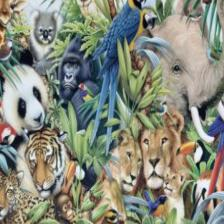
\includegraphics[width=0.14\linewidth]{figs/splash/original} &
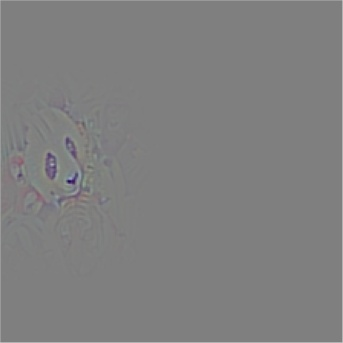
\includegraphics[width=0.14\linewidth]{figs/splash/panda} &
\includegraphics[width=0.14\linewidth]{figs/splash/tiger} &
\includegraphics[width=0.14\linewidth]{figs/splash/gorilla} &
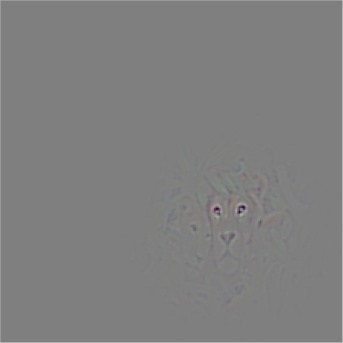
\includegraphics[width=0.14\linewidth]{figs/splash/lion} &
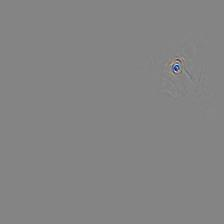
\includegraphics[width=0.14\linewidth]{figs/splash/elephant} &
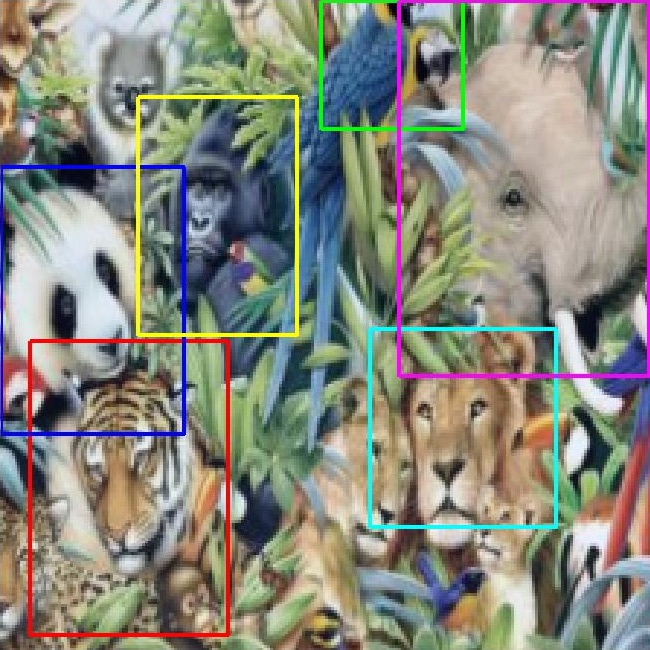
\includegraphics[width=0.14\linewidth]{figs/splash/localization}\\
{\small (a) Input Image} &
{\small (b) Panda} &
{\small (c) Tiger} &
{\small (d) Gorilla} &
{\small (e) Lion} &
{\small (f) Elephant} &
{\small (g) Localization}
\end{tabular}
\caption{We illustrate the localization power of the feedback net on a multi-object image with cluttered background. (a) shows the original input image which both VggNet~\cite{Simonyan2014Very} and GoogleNet~\cite{Szegedy2014Going} recognize as "comic book". (b) - (f) illustrate our feedback model on understanding the image given different class labels as a prior. We visualize the gradient of each class node with respect to image after the feedback net finish its inference. (g) shows the final localizations for different objects based on the gradients. Better viewed in color.}
\label{fig:splah}
\end{center}
\end{figure*}

\textbf{Optimization in a Feedback Loop}:
% Explain from the machine learning perspective
From a machine learning perspective, the proposed feedback networks \emph{add extra flexibility to Convolutional Networks, to help in capturing visual attention and improving feature detection}. Convolutional Neural Networks~\cite{lecun1998gradient, Krizhevsky2012ImageNet, Simonyan2014Very} have achieved great success in both machine learning and computer vision in recent years. Benefiting from large-scale training data, (\emph{e.g.,} ImageNet~\cite{deng2009imagenet}), CNNs are capable of learning filters and image compositions at the same time. Various approaches have been adopted to further increase generalization ability of CNNs, by either adding regularization in training~\cite{he2015delving,ioffe2015batch}, or going deeper~\cite{Simonyan2014Very, Szegedy2014Going}. Inspired by Deformable Part-Based Models (DPMs)~\cite{Felzenszwalb2010Object} that characterize middle level part locations as latent variables and search for them during object detection, we utilize a simple yet efficient method to optimize image compositions and assign neuron activations given ``goals'' in visual search. The algorithm maximizes the posterior response of network given target high-level semantic concepts, in a top-down manner. Compared with traditional bottom-up strategies~\cite{he2015delving, ioffe2015batch}, which aim to regularize the network training, the proposed feedback framework adds flexibilities to the model inference from high-level concepts down to the receptive field.

Figure~\ref{fig:splah} shows an example on how this flexibility is reflected in detection and localization. Instead of recognizing the input image as a ``comic book'', the proposed feedback network is capable to localize each component of the ``comic book'' via salience maps. The example shown in Figure~\ref{fig:splash0} illustrates its working mechanism: given a high-level semantic stimulus ``PANDA'', only the neurons in hidden layers related with the concept ``PANDA'' will be activated by iterative optimization in a feedback loop. As a result, only salient regions related with the concept ``PANDA'' are captured in visualizations.
As suggested by those results, the feedback networks achieve certain level of selectivity and provide non-relevant suppression during the top-down inference, allowing the model to focus on the most salient image regions that improve the class confidence.

% Unify the network: recognition and detection in a single network.
% Simultaneously answer the question of "what" and "where"
\textbf{Weakly Supervised Object Localization}:
Given gradient visualizations in Figure~\ref{fig:splah}, we further develop an algorithm for weakly supervised object localization. Instead of using large amount of supervision (\emph{e.g.}, bounding box positions) in traditional methods such as R-CNN~\cite{girshick2014rich} or using regression model~\cite{erhan2014scalable, Simonyan2014Very}, we don't require any localization information in the training stage. Instead, we adopt \emph{a unified network performing both recognition and localization tasks}, to answer questions of ``what'' and ``where'' simultaneously, which are the two most important tasks in computer vision. Experimental results suggest that our weakly supervised algorithm using feedback network could achieve similar performance on ImageNet object localization task as GoogLeNet~\cite{Szegedy2014Going} and VGG~\cite{Simonyan2014Very}.

% Newly added to say something about the classification task
\textbf{Image Classification Revisited}:
We mimic the human visual recognition process that human may focus to recognize objects in a complicated image after a first time glimpse as the procedure ``Look and Think Twice'' for image classification. We utilize the weakly supervised object localization during the ``first glimpse'' to make guesses of ROIs, then make the network refocused on those ROIs and give final classifications list. Experimental results on ImageNet 2014 classification validation dataset suggest that this approach is efficient to eliminate irrelevant clutters and improve classification accuracy especially on small objects.


%\setlength{\tabcolsep}{2pt}
%\begin{figure*}
%\begin{center}
%\begin{tabular}{ccccccccc}
%\rotatebox{90}{\hspace{5mm}Oxford} &
%\includegraphics[width=0.11\linewidth]{figs/visual_compare/gradient/oxford/panda} &
%\includegraphics[width=0.11\linewidth]{figs/visual_compare/saliency/oxford/panda} &
%\includegraphics[width=0.11\linewidth]{figs/visual_compare/gradient/oxford/tiger} &
%\includegraphics[width=0.11\linewidth]{figs/visual_compare/saliency/oxford/tiger} &
%\includegraphics[width=0.11\linewidth]{figs/visual_compare/gradient/oxford/gorilla} &
%\includegraphics[width=0.11\linewidth]{figs/visual_compare/saliency/oxford/gorilla} &
%\includegraphics[width=0.11\linewidth]{figs/visual_compare/gradient/oxford/lion} &
%\includegraphics[width=0.11\linewidth]{figs/visual_compare/saliency/oxford/lion} \\
%\rotatebox{90}{\hspace{5mm}Deconv} &
%\includegraphics[width=0.11\linewidth]{figs/visual_compare/gradient/deconv/panda} &
%\includegraphics[width=0.11\linewidth]{figs/visual_compare/saliency/deconv/panda} &
%\includegraphics[width=0.11\linewidth]{figs/visual_compare/gradient/deconv/tiger} &
%\includegraphics[width=0.11\linewidth]{figs/visual_compare/saliency/deconv/tiger} &
%\includegraphics[width=0.11\linewidth]{figs/visual_compare/gradient/deconv/gorilla} &
%\includegraphics[width=0.11\linewidth]{figs/visual_compare/saliency/deconv/gorilla} &
%\includegraphics[width=0.11\linewidth]{figs/visual_compare/gradient/deconv/lion} &
%\includegraphics[width=0.11\linewidth]{figs/visual_compare/saliency/deconv/lion} \\
%\rotatebox{90}{\hspace{5mm}Our} &
%\includegraphics[width=0.11\linewidth]{figs/visual_compare/gradient/feedback/panda} &
%\includegraphics[width=0.11\linewidth]{figs/visual_compare/saliency/feedback/panda} &
%\includegraphics[width=0.11\linewidth]{figs/visual_compare/gradient/feedback/tiger} &
%\includegraphics[width=0.11\linewidth]{figs/visual_compare/saliency/feedback/tiger} &
%\includegraphics[width=0.11\linewidth]{figs/visual_compare/gradient/feedback/gorilla} &
%\includegraphics[width=0.11\linewidth]{figs/visual_compare/saliency/feedback/gorilla} &
%\includegraphics[width=0.11\linewidth]{figs/visual_compare/gradient/feedback/lion} &
%\includegraphics[width=0.11\linewidth]{figs/visual_compare/saliency/feedback/lion} \\
%&
%\multicolumn{2}{c}{{\small (a) Panda}} &
%\multicolumn{2}{c}{{\small (b) Tiger}} &
%\multicolumn{2}{c}{{\small (c) Gorilla}} &
%\multicolumn{2}{c}{{\small (d) Lion}} \\
%\end{tabular}
%% \vspace{-10pt}
%\caption{We demonstrate the effectiveness of our method by comparing the class model visualization results against Oxford~\cite{simonyan2013deep} and Deconv~\cite{zeiler2014visualizing}. The input image is the same as Figure 1 (a). We show both the visualization results as well as the saliency map. While both Oxford and Deconv have the same input: the image and an object class label (i.e. tiger, panda, etc.), the gradients computed are often salient on one particular object (i.e. elephant). Our feedback framework allows for the model to focus on the most important image area that improves the class confidence.}
%\label{fig:visual_compare}
%% \vspace{-30pt}
%\end{center}
%\end{figure*}
